\documentclass[aspectratio=169]{beamer}

% Packages
\usepackage{graphicx}
\usepackage{tikz}
\usetikzlibrary{shapes.geometric, arrows.meta, positioning, fit, backgrounds, calc}
\usepackage{booktabs}
\usepackage{pifont} % for \ding{51} and \ding{55}

% Custom restrained academic palette
\definecolor{navy}{RGB}{20, 30, 60}
\definecolor{charcoal}{RGB}{50, 50, 50}
\definecolor{accent}{RGB}{0, 102, 204}
\definecolor{errorred}{RGB}{200, 40, 40}
\definecolor{successgreen}{RGB}{40, 140, 60}

% Theme configuration
\usetheme{default}
\usefonttheme{default}
\setbeamercolor{structure}{fg=navy}
\setbeamercolor{title}{fg=navy}
\setbeamercolor{frametitle}{fg=navy, bg=white}
\setbeamercolor{normal text}{fg=charcoal}
\setbeamercolor{itemize item}{fg=accent}

\setbeamertemplate{navigation symbols}{} % clean layout
\setbeamertemplate{footline}[frame number] % minimal footer
\setbeamertemplate{frametitle}{\vspace{0.5cm}\Large\bfseries\insertframetitle}

\begin{document}

% =========================================================
% PRESENTER 1: ABDUL MOMIT TALUKDER
% Slides 1 - 6
% =========================================================

% SLIDE 1
\begin{frame}[plain]
    \begin{center}
        \vspace{0.8cm}
        {\Huge \bfseries \textcolor{navy}{Signal-Aware ML Calibration for\\[0.2cm] Low-Cost Pan-Tilt LiDAR}} \\[0.6cm]
        {\Large Undergraduate Thesis Proposal} \\[0.2cm]
        {\large CSE 4100: Project or Thesis with Seminar Part I} \\[0.8cm]
        
        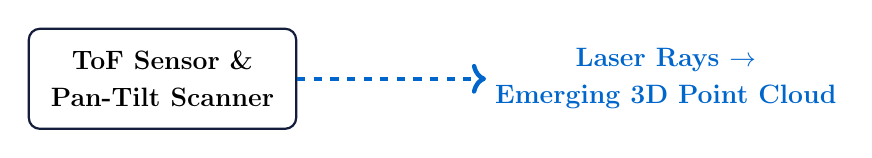
\begin{tikzpicture}[scale=0.8, transform shape]
            \node[draw=navy, thick, rounded corners, inner sep=10pt, align=center, font=\large\bfseries] (sensor) {ToF Sensor \&\\[0.1cm]Pan-Tilt Scanner};
            \draw[->, accent, ultra thick, dashed] (sensor.east) -- ++(3,0) node[right, align=center, font=\large\bfseries] {Laser Rays $\rightarrow$ \\[0.1cm] Emerging 3D Point Cloud};
        \end{tikzpicture}\\[0.8cm]

        {\small 
        \textbf{Students:} Abdul Momit Talukder (232311320) | Oishi Farzana (232311294) | Mahfuz Ahmad (232311307) \\[0.1cm]
        \textbf{Supervisor:} Mohd Ruhul Ameen, Lecturer \\[0.1cm]
        Department of Computer Science and Engineering | Varendra University | 7th Semester | Section E
        }
    \end{center}
\end{frame}

% SLIDE 2
\begin{frame}{How Do Machines ``See'' 3D?}
    \begin{center}
        \vspace{0.5cm}
        {\Huge \textbf{\textcolor{navy}{Distance + Direction $\rightarrow$ 3D Geometry}}}
        
        \vspace{1.5cm}
        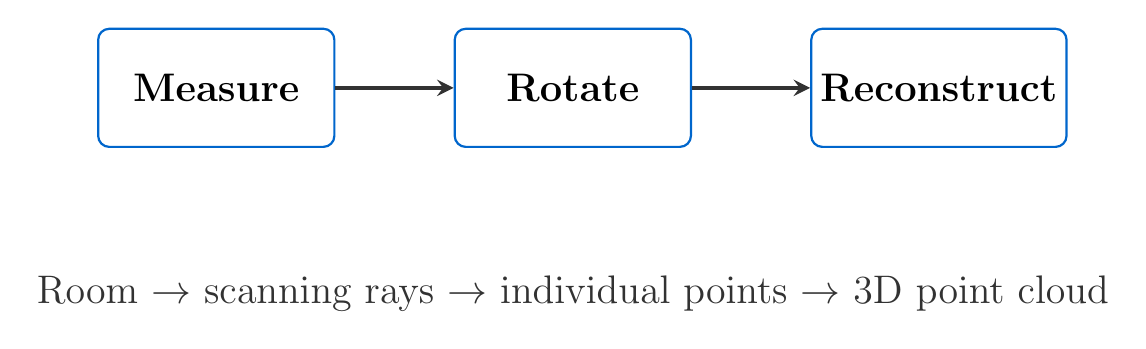
\begin{tikzpicture}[
            box/.style={draw=accent, thick, rounded corners, minimum width=3cm, minimum height=1.5cm, align=center, font=\Large\bfseries},
            arrow/.style={->, >=stealth, ultra thick, charcoal}
        ]
            \node[box] (measure) {Measure};
            \node[box, right=1.5cm of measure] (rotate) {Rotate};
            \node[box, right=1.5cm of rotate] (reconstruct) {Reconstruct};
            
            \draw[arrow] (measure) -- (rotate);
            \draw[arrow] (rotate) -- (reconstruct);
            
            \node[below=1.5cm of rotate, text=charcoal, font=\Large] (room) {Room $\rightarrow$ scanning rays $\rightarrow$ individual points $\rightarrow$ 3D point cloud};
        \end{tikzpicture}
    \end{center}
\end{frame}

% SLIDE 3
\begin{frame}{3D Sensing Is Powerful — But Expensive}
    \vspace{0.5cm}
    \begin{columns}
        \column{0.5\textwidth}
        \begin{center}
            {\fontsize{50}{60}\selectfont \bfseries \textcolor{errorred}{\$500+}} \\[0.5cm]
            {\Large Commercial LiDAR}
        \end{center}
        \column{0.5\textwidth}
        \begin{center}
            {\fontsize{50}{60}\selectfont \bfseries \textcolor{successgreen}{$\sim$\$25}} \\[0.5cm]
            {\Large Our Target}
        \end{center}
    \end{columns}
    \vspace{2cm}
    \begin{center}
        {\Large \bfseries High performance is expensive. \\[0.2cm]
        Low cost often means lower accuracy.}
    \end{center}
\end{frame}

% SLIDE 4
\begin{frame}{Why Time-of-Flight?}
    \vspace{1cm}
    \begin{columns}[t]
        \column{0.33\textwidth}
        \begin{center}
            {\Large \bfseries Ultrasonic} \\[0.8cm]
            \textcolor{errorred}{\ding{55}} Wide beam \\[0.3cm]
            \textcolor{errorred}{\ding{55}} Lower spatial resolution
        \end{center}
        
        \column{0.33\textwidth}
        \begin{center}
            {\Large \bfseries Radar} \\[0.8cm]
            \textcolor{errorred}{\ding{55}} Strong indoor complexity
        \end{center}
        
        \column{0.33\textwidth}
        \begin{center}
            {\Large \bfseries \textcolor{accent}{Time-of-Flight}} \\[0.8cm]
            \textcolor{successgreen}{\ding{51}} Compact \\[0.3cm]
            \textcolor{successgreen}{\ding{51}} Fast \\[0.3cm]
            \textcolor{successgreen}{\ding{51}} Fine spatial sensing
        \end{center}
    \end{columns}
\end{frame}

% SLIDE 5
\begin{frame}{Our Hardware Architecture}
    \begin{center}
        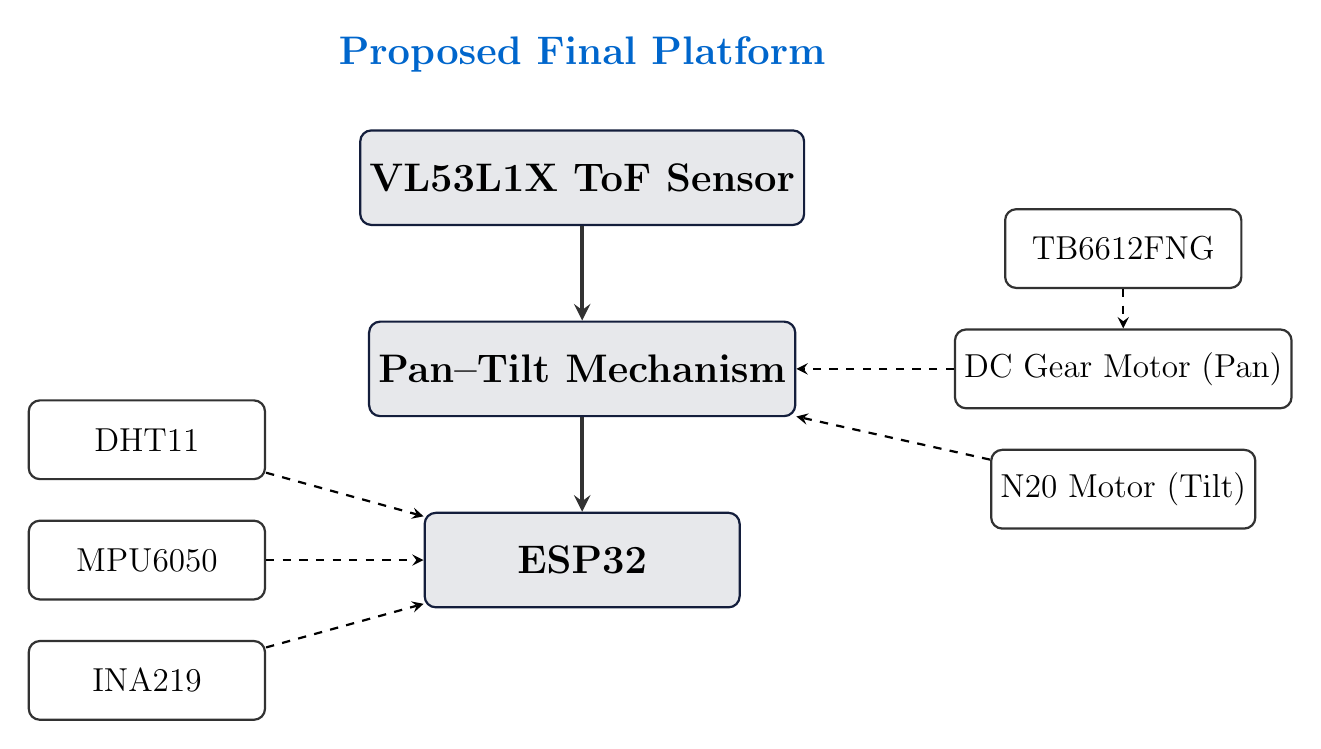
\begin{tikzpicture}[
            node distance=1.2cm,
            mainbox/.style={draw=navy, thick, fill=navy!10, rounded corners, minimum width=4cm, minimum height=1.2cm, align=center, font=\Large\bfseries},
            subbox/.style={draw=charcoal, thick, rounded corners, minimum width=3cm, minimum height=1cm, align=center, font=\large},
            arrow/.style={->, >=stealth, ultra thick, charcoal}
        ]
            % Main vertical pipeline
            \node[mainbox] (sensor) {VL53L1X ToF Sensor};
            \node[mainbox, below=1.2cm of sensor] (pantilt) {Pan--Tilt Mechanism};
            \node[mainbox, below=1.2cm of pantilt] (esp) {ESP32};
            
            \draw[arrow] (sensor) -- (pantilt);
            \draw[arrow] (pantilt) -- (esp);
            
            % Supporting sensors
            \node[subbox, left=2cm of esp] (mpu) {MPU6050};
            \node[subbox, above=0.5cm of mpu] (dht) {DHT11};
            \node[subbox, below=0.5cm of mpu] (ina) {INA219};
            
            \draw[->, >=stealth, thick, dashed] (mpu) -- (esp);
            \draw[->, >=stealth, thick, dashed] (dht) -- (esp);
            \draw[->, >=stealth, thick, dashed] (ina) -- (esp);
            
            % Motors
            \node[subbox, right=2cm of pantilt] (dc) {DC Gear Motor (Pan)};
            \node[subbox, above=0.5cm of dc] (driver) {TB6612FNG};
            \node[subbox, below=0.5cm of dc] (n20) {N20 Motor (Tilt)};
            
            \draw[->, >=stealth, thick, dashed] (dc) -- (pantilt);
            \draw[->, >=stealth, thick, dashed] (n20) -- (pantilt);
            \draw[->, >=stealth, thick, dashed] (driver) -- (dc);
            
            \node[above=0.6cm of sensor, text=accent, font=\Large\bfseries] {Proposed Final Platform};
            
        \end{tikzpicture}
    \end{center}
\end{frame}

% SLIDE 6
\begin{frame}{From Concept to Pilot}
    \vspace{0.5cm}
    \begin{columns}
        \column{0.5\textwidth}
        \begin{center}
            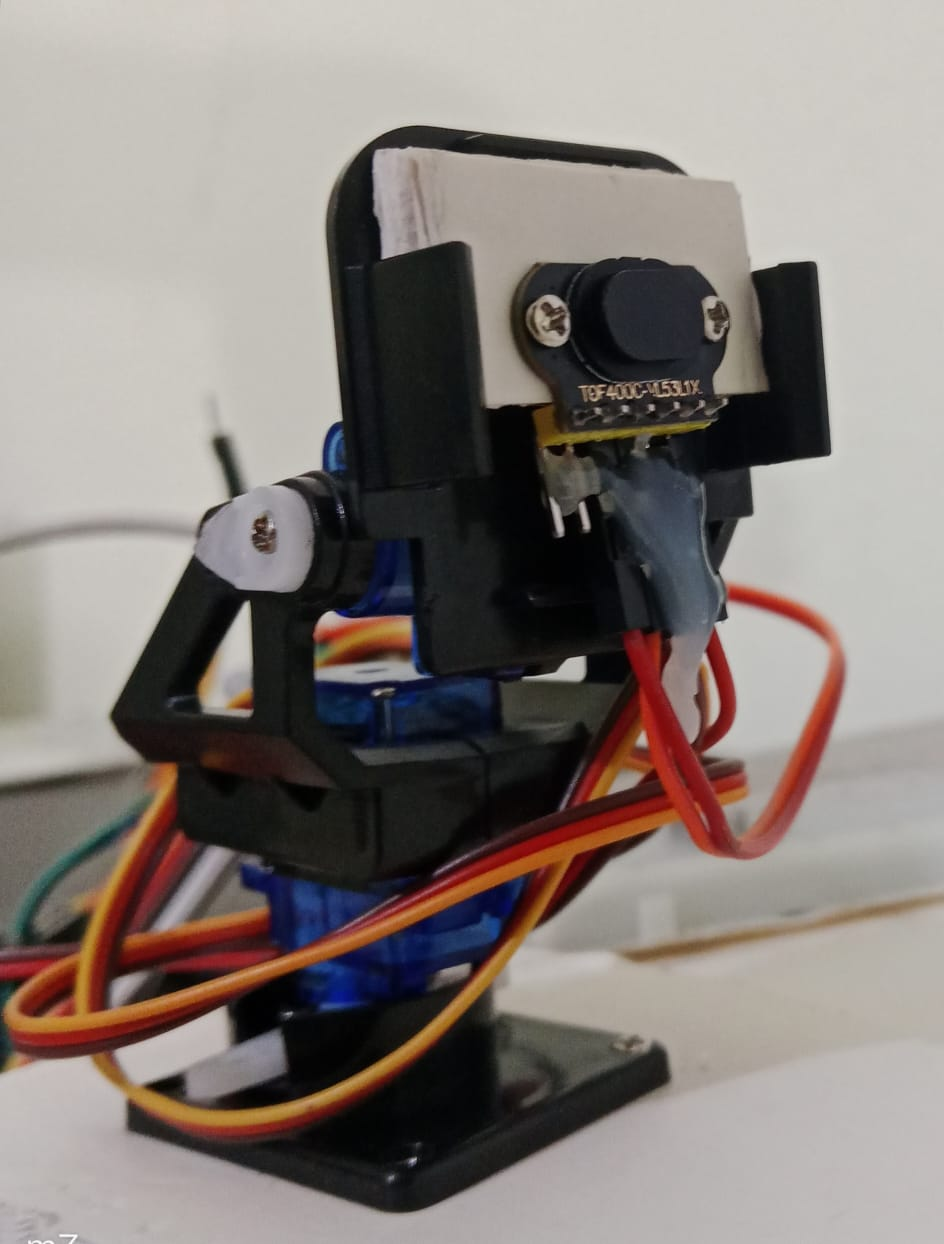
\includegraphics[height=5.5cm, keepaspectratio]{figures/hardware_setup.png} \\[0.3cm]
            {\footnotesize \textcolor{charcoal}{Preliminary SG90-based prototype used for pilot data collection}}
        \end{center}
        \column{0.5\textwidth}
        \begin{center}
            {\fontsize{45}{55}\selectfont \bfseries \textcolor{accent}{68,000+}} \\[0.5cm]
            {\Large pilot measurements} \\[1cm]
            {\Large 2 indoor campaigns} \\[1.5cm]
            \textcolor{charcoal}{\textbf{\textit{Pilot prototype $\neq$ Final thesis platform}}}
        \end{center}
    \end{columns}
\end{frame}

% =========================================================
% PRESENTER 2: OISHI FARZANA
% Slides 7 - 11
% =========================================================

% SLIDE 7
\begin{frame}{Scan $\rightarrow$ Measure $\rightarrow$ Repeat $\rightarrow$ Reconstruct}
    \begin{center}
        \vspace{1cm}
        
\begin{tikzpicture}[
            box/.style={draw=accent, thick, rounded corners, minimum width=2.2cm, minimum height=1.2cm, align=center, font=\Large\bfseries},
            arrow/.style={->, >=stealth, ultra thick, charcoal}
        ]
            \node[box] (pan) {Pan};
            \node[box, right=0.8cm of pan] (tilt) {Tilt};
            \node[box, right=0.8cm of tilt] (measure) {Measure};
            \node[box, right=0.8cm of measure] (point) {Point};
            \node[box, right=0.8cm of point] (repeat) {Repeat};
            
            \draw[arrow] (pan) -- (tilt);
            \draw[arrow] (tilt) -- (measure);
            \draw[arrow] (measure) -- (point);
            \draw[arrow] (point) -- (repeat);
        \end{tikzpicture}
        
        \vspace{2cm}
        {\Huge \bfseries \textcolor{navy}{Hundreds of points $\rightarrow$ 3D room}} \\[1.5cm]
        {\Large \textcolor{charcoal}{Each distance measurement becomes one 3D point.}}
    \end{center}
\end{frame}

% SLIDE 8
\begin{frame}{The Real World Is Messy}
    \vspace{0.5cm}
    \begin{columns}
        \column{0.33\textwidth}
        \begin{center}
            
\begin{tikzpicture}
                \fill[charcoal] (0,0) rectangle (2.5,2);
                \draw[->, ultra thick, errorred] (-1.5, 1) -- (0, 1) node[midway, above] {\small Laser};
            \end{tikzpicture}\\[0.8cm]
            {\Large \bfseries Weak Return} \\[0.2cm]
            \large Dark Surface
        \end{center}
        \column{0.33\textwidth}
        \begin{center}
            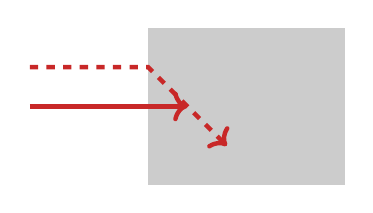
\begin{tikzpicture}
                \fill[gray!40] (0,0) rectangle (2.5,2);
                \draw[->, ultra thick, errorred] (-1.5, 1) -- (0.5, 1);
                \draw[->, ultra thick, errorred, dashed] (-1.5, 1.5) -- (0, 1.5) -- (1, 0.5);
            \end{tikzpicture}\\[0.8cm]
            {\Large \bfseries Mixed Returns} \\[0.2cm]
            \large Reflective Surface
        \end{center}
        \column{0.33\textwidth}
        \begin{center}
            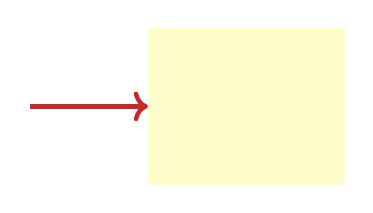
\begin{tikzpicture}
                \fill[yellow!20] (0,0) rectangle (2.5,2);
                \draw[->, ultra thick, errorred] (-1.5, 1) -- (0, 1);
                \node at (1.25, 1) {\Huge \textcolor{orange}{$\bigstar$}};
            \end{tikzpicture}\\[0.8cm]
            {\Large \bfseries Ambient Noise} \\[0.2cm]
            \large Bright Room
        \end{center}
    \end{columns}
    \vspace{1.8cm}
    \begin{center}
        {\Huge \bfseries \textcolor{errorred}{$\rightarrow$ Range Error}}
    \end{center}
\end{frame}

% SLIDE 9
\begin{frame}{Scale the Evidence}
    \begin{center}
        \vspace{0.5cm}
        {\fontsize{50}{60}\selectfont \bfseries \textcolor{accent}{150,000+}} \\[0.5cm]
        {\Large measurements} \\[1.5cm]
        
        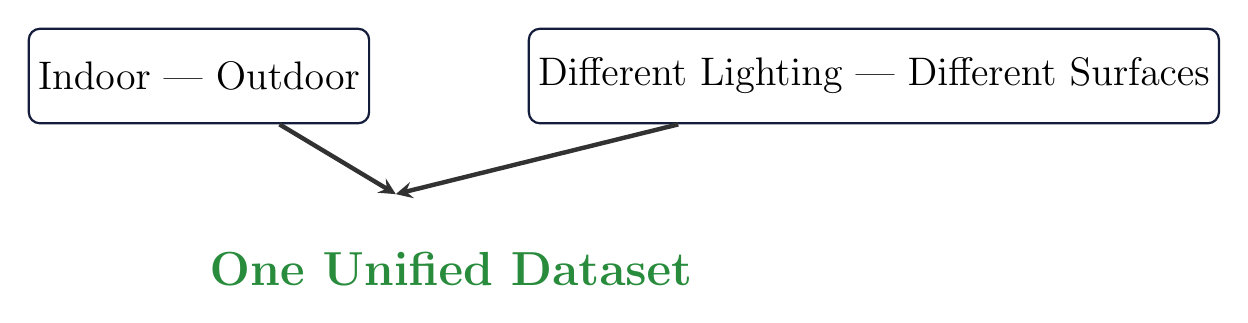
\begin{tikzpicture}[
            node distance=1.5cm,
            box/.style={draw=navy, thick, rounded corners, minimum width=4cm, minimum height=1.2cm, align=center, font=\Large}
        ]
            \node[box] (indoor) {Indoor | Outdoor};
            \node[box, right=2cm of indoor] (lighting) {Different Lighting | Different Surfaces};
            
            \draw[->, >=stealth, ultra thick, charcoal] (indoor) -- (2.5, -1.5);
            \draw[->, >=stealth, ultra thick, charcoal] (lighting) -- (2.5, -1.5);
            
            \node[below=1.5cm of indoor, xshift=3.2cm, font=\LARGE\bfseries\color{successgreen}] (dataset) {One Unified Dataset};
        \end{tikzpicture} \\[1.5cm]
        
        \textcolor{charcoal}{\Large \textit{Paired with ground-truth measurements}}
    \end{center}
\end{frame}

% SLIDE 10
\begin{frame}{Will It Work in a New Environment?}
    \begin{center}
        \vspace{0.5cm}
        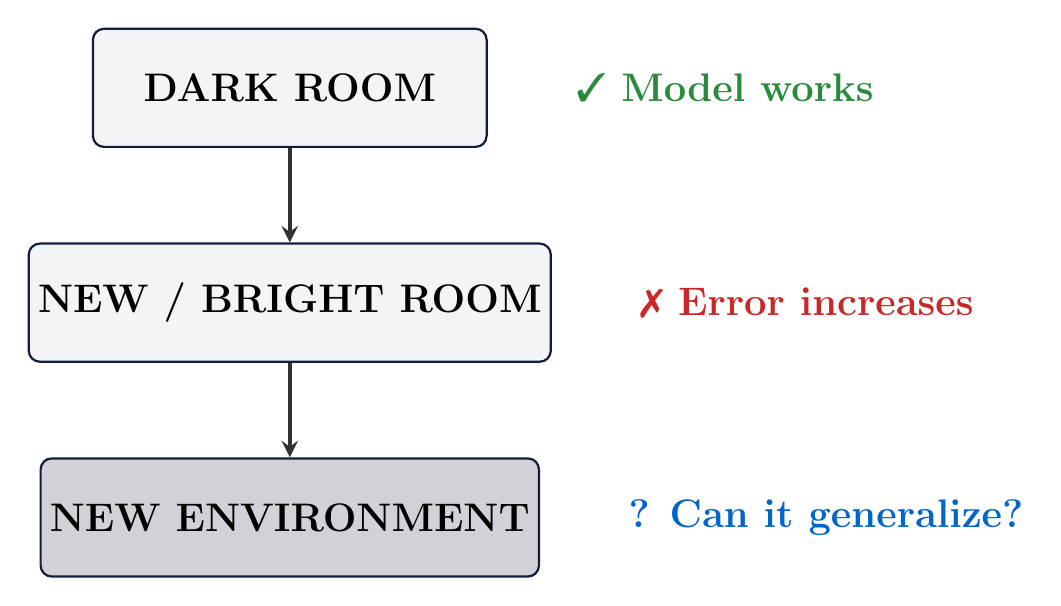
\begin{tikzpicture}[
            box/.style={draw=navy, thick, fill=navy!5, rounded corners, minimum width=5cm, minimum height=1.5cm, align=center, font=\Large\bfseries}
        ]
            \node[box] (dark) {DARK ROOM};
            \node[right=1cm of dark, text=successgreen, font=\Large\bfseries] (check) {\ding{51} Model works};
            
            \node[box, below=1.2cm of dark] (bright) {NEW / BRIGHT ROOM};
            \node[right=1cm of bright, text=errorred, font=\Large\bfseries] (cross) {\ding{55} Error increases};
            
            \node[box, fill=navy!20, below=1.2cm of bright] (new) {NEW ENVIRONMENT};
            \node[right=1cm of new, text=accent, font=\Large\bfseries] (question) {\textbf{?} Can it generalize?};
            
            \draw[->, >=stealth, ultra thick, charcoal] (dark) -- (bright);
            \draw[->, >=stealth, ultra thick, charcoal] (bright) -- (new);
        \end{tikzpicture}
    \end{center}
\end{frame}

% SLIDE 11
\begin{frame}{Democratizing 3D Sensing}
    \vspace{1cm}
    \begin{columns}[t]
        \column{0.33\textwidth}
        \begin{center}
            {\Large \bfseries \textcolor{accent}{Education}} \\[0.8cm]
            \large Affordable research
        \end{center}
        \column{0.33\textwidth}
        \begin{center}
            {\Large \bfseries \textcolor{accent}{Robotics}} \\[0.8cm]
            \large Low-cost spatial awareness
        \end{center}
        \column{0.33\textwidth}
        \begin{center}
            {\Large \bfseries \textcolor{accent}{Assistive Technology}} \\[0.8cm]
            \large Obstacle/environment sensing
        \end{center}
    \end{columns}
    \vspace{2.5cm}
    \begin{center}
        {\LARGE \bfseries \textcolor{navy}{Advanced sensing should not require expensive hardware.}}
    \end{center}
\end{frame}

% =========================================================
% PRESENTER 3: MAHFUZ AHMAD
% Slides 12 - 16
% =========================================================

% SLIDE 12
\begin{frame}{Don't Use Distance Alone}
    \begin{center}
        \vspace{0.2cm}
        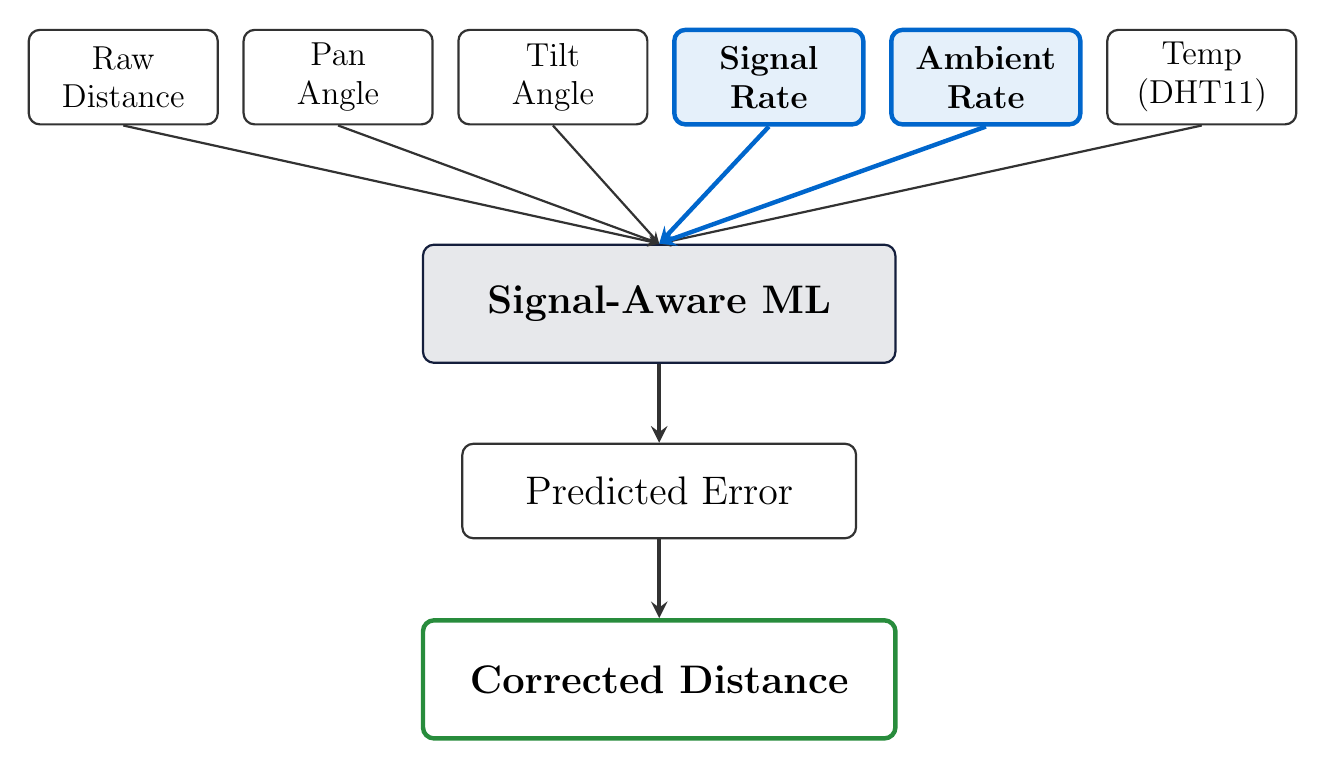
\begin{tikzpicture}[
            feat/.style={draw=charcoal, thick, rounded corners, minimum height=1.2cm, minimum width=2.4cm, align=center, font=\large},
            highlight/.style={draw=accent, ultra thick, fill=accent!10, rounded corners, minimum height=1.2cm, minimum width=2.4cm, align=center, font=\large\bfseries}
        ]
            % Features
            \node[feat] (raw) {Raw\\Distance};
            \node[feat, right=0.3cm of raw] (pan) {Pan\\Angle};
            \node[feat, right=0.3cm of pan] (tilt) {Tilt\\Angle};
            
            \node[highlight, right=0.3cm of tilt] (sig) {Signal\\Rate};
            \node[highlight, right=0.3cm of sig] (amb) {Ambient\\Rate};
            
            \node[feat, right=0.3cm of amb] (temp) {Temp\\(DHT11)};
            
            % ML Node
            \node[draw=navy, thick, fill=navy!10, minimum width=6cm, minimum height=1.5cm, rounded corners, font=\Large\bfseries, below=1.5cm of tilt, xshift=1.35cm] (ml) {Signal-Aware ML};
            
            % Output Nodes
            \node[draw=charcoal, thick, minimum width=5cm, minimum height=1.2cm, rounded corners, font=\Large, below=1cm of ml] (err) {Predicted Error};
            
            \node[draw=successgreen, ultra thick, minimum width=6cm, minimum height=1.5cm, rounded corners, font=\Large\bfseries, below=1cm of err] (corr) {Corrected Distance};
            
            % Arrows
            \draw[->, >=stealth, thick, charcoal] (raw.south) -- (ml.north);
            \draw[->, >=stealth, thick, charcoal] (pan.south) -- (ml.north);
            \draw[->, >=stealth, thick, charcoal] (tilt.south) -- (ml.north);
            \draw[->, >=stealth, thick, charcoal] (temp.south) -- (ml.north);
            
            \draw[->, >=stealth, ultra thick, accent] (sig.south) -- (ml.north);
            \draw[->, >=stealth, ultra thick, accent] (amb.south) -- (ml.north);
            
            \draw[->, >=stealth, ultra thick, charcoal] (ml.south) -- (err.north);
            \draw[->, >=stealth, ultra thick, charcoal] (err.south) -- (corr.north);
            
        \end{tikzpicture}
    \end{center}
\end{frame}

% SLIDE 13
\begin{frame}{From Python to ESP32}
    \begin{center}
        \vspace{1cm}
        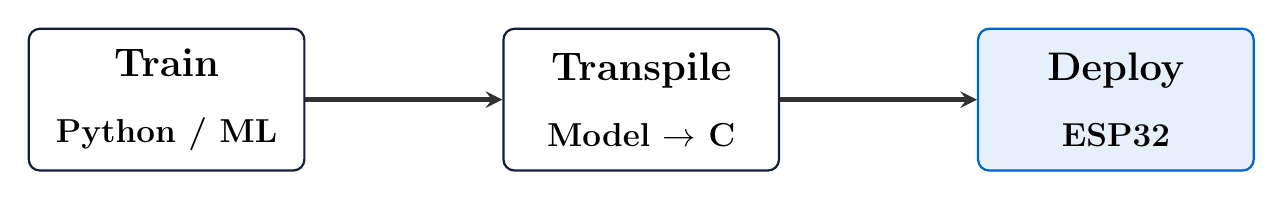
\begin{tikzpicture}[
            node distance=2.5cm,
            box/.style={draw=navy, thick, rounded corners, minimum width=3.5cm, minimum height=1.8cm, align=center, font=\Large\bfseries},
            arrow/.style={->, >=stealth, ultra thick, charcoal}
        ]
            \node[box] (train) {Train\\[0.2cm] \large Python / ML};
            \node[box, right=of train] (transpile) {Transpile\\[0.2cm] \large Model $\rightarrow$ C};
            \node[box, draw=accent, fill=accent!10, right=of transpile] (deploy) {Deploy\\[0.2cm] \large ESP32};
            
            \draw[arrow] (train) -- (transpile);
            \draw[arrow] (transpile) -- (deploy);
        \end{tikzpicture}
        
        \vspace{2cm}
        {\Huge \bfseries \textcolor{accent}{$<$ 100 $\mu$s}} \\[0.3cm]
        {\Large inference target} \\[0.8cm]
        {\Large \textcolor{charcoal}{Zero external runtime dependency}}
    \end{center}
\end{frame}

% SLIDE 14
\begin{frame}{Pilot Results: Promising, but Not Final}
    \vspace{1cm}
    \begin{columns}
        \column{0.5\textwidth}
        \begin{center}
            {\fontsize{50}{60}\selectfont \bfseries \textcolor{successgreen}{94.7\%}} \\[0.5cm]
            {\Large MAE reduction} \\[0.2cm]
            {\large Day 2 pilot}
        \end{center}
        \column{0.5\textwidth}
        \begin{center}
            {\fontsize{50}{60}\selectfont \bfseries \textcolor{accent}{22.4 mm}} \\[0.5cm]
            {\Large MAE} \\[0.2cm]
            {\large pooled pilot training}
        \end{center}
    \end{columns}
    
    \vspace{2.5cm}
    
    \begin{center}
        \textcolor{errorred}{\normalsize \textbf{*} Pilot results; final evaluation will use corrected ground truth and scan-level validation.}
    \end{center}
\end{frame}

% SLIDE 15
\begin{frame}{From Pilot $\rightarrow$ Robust System}
    \begin{center}
        \vspace{1.5cm}
        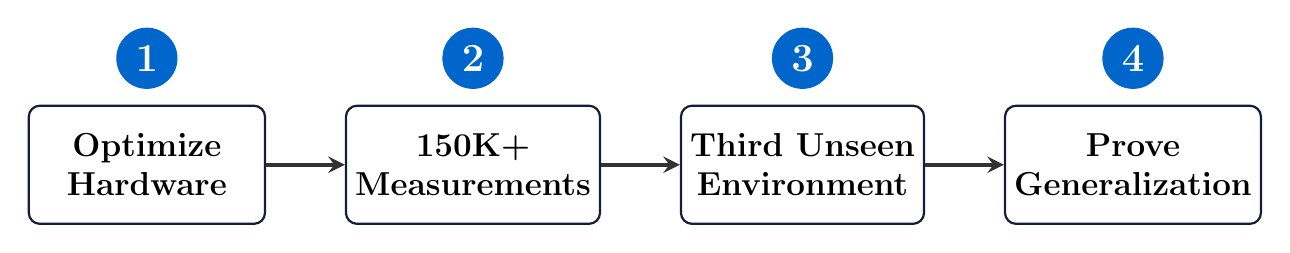
\begin{tikzpicture}[
            node distance=1cm,
            box/.style={draw=navy, thick, rounded corners, minimum width=3cm, minimum height=1.5cm, align=center, font=\large\bfseries},
            num/.style={circle, draw=accent, fill=accent, text=white, font=\Large\bfseries},
            arrow/.style={->, >=stealth, ultra thick, charcoal}
        ]
            \node[box] (step1) {Optimize\\Hardware};
            \node[num, above=0.2cm of step1] {1};
            
            \node[box, right=of step1] (step2) {150K+\\Measurements};
            \node[num, above=0.2cm of step2] {2};
            
            \node[box, right=of step2] (step3) {Third Unseen\\Environment};
            \node[num, above=0.2cm of step3] {3};
            
            \node[box, right=of step3] (step4) {Prove\\Generalization};
            \node[num, above=0.2cm of step4] {4};
            
            \draw[arrow] (step1) -- (step2);
            \draw[arrow] (step2) -- (step3);
            \draw[arrow] (step3) -- (step4);
        \end{tikzpicture}
        
        \vspace{2cm}
        {\Large \bfseries \textcolor{navy}{Final 3D reconstruction + ESP32 deployment}}
    \end{center}
\end{frame}

% SLIDE 16
\begin{frame}{Built to Be Shared}
    \vspace{1cm}
    \begin{columns}[t]
        \column{0.33\textwidth}
        \begin{center}
            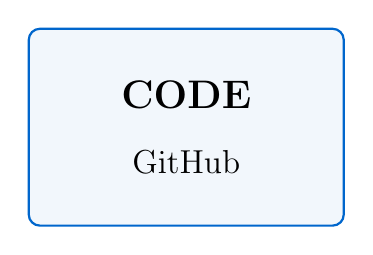
\begin{tikzpicture}\node[draw=accent, thick, fill=accent!5, rounded corners, minimum width=4cm, minimum height=2.5cm, align=center] {\Large \bfseries CODE \\[0.4cm] \large GitHub};\end{tikzpicture}
        \end{center}
        \column{0.33\textwidth}
        \begin{center}
            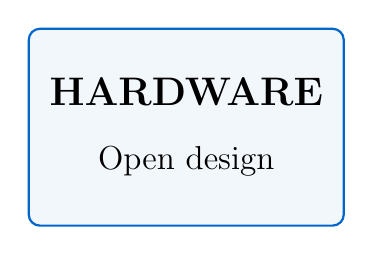
\begin{tikzpicture}\node[draw=accent, thick, fill=accent!5, rounded corners, minimum width=4cm, minimum height=2.5cm, align=center] {\Large \bfseries HARDWARE \\[0.4cm] \large Open design};\end{tikzpicture}
        \end{center}
        \column{0.33\textwidth}
        \begin{center}
            
\begin{tikzpicture}\node[draw=accent, thick, fill=accent!5, rounded corners, minimum width=4cm, minimum height=2.5cm, align=center] {\Large \bfseries DATA \\[0.4cm] \large Public dataset};\end{tikzpicture}
        \end{center}
    \end{columns}
    
    \vspace{1.5cm}
    \begin{center}
        {\LARGE \bfseries \textcolor{navy}{Low-cost sensing. Reproducible research. Open access.}} \\[1cm]
        {\Huge \bfseries Thank You} \\[0.5cm]
        {\Large Questions?}
    \end{center}
\end{frame}

\end{document}
